
\section{Abstract Factory}
\textbf{Kategorie}: Creational

Definiert Schnittstelle zur Erzeugung einer Familie von Objekten, wobei die konkreten Klassen der zu instanziierenden Objekten nicht näher festgelegt werden.

\textbf{Verwenden wenn}:

\begin{itemize}
	\item ein System unabhängig von der Art der Erzeugung seiner Produkte arbeiten soll
	\item ein System mit einer oder mehreren Produktefamilien konfiguriert werden soll
	\item eine Gruppe von Produkten gemeinsam genutzt werden soll
	\item in einer Library die Schnittstellen von Produkten ohne deren Implementierung bereitgestellt werden soll
\end{itemize}

\begin{itemize}
	\item \textit{Typische Anwendung}: Erstellung eines GUI mit versch. Themes
\end{itemize}

\begin{figure}[H]
	\centering
	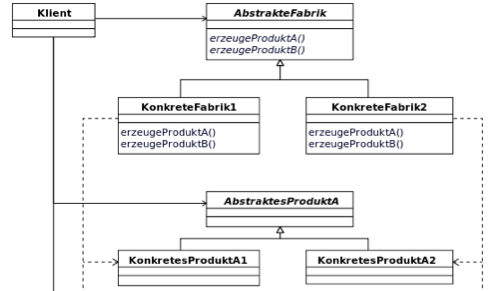
\includegraphics[width=0.9\textwidth]{content/gof/images/01-abstract-factory-uml.png}
	\caption{Abstract Factory UML}
\end{figure}


\section{Prototype}
\textbf{Kategorie}: Creational

Wenn der Typ eines Objeckts aufgrund einer Prototypen-Instanz bestimmt wird. Diese wird geklont um neue Objekte zu erstellen. Dies ermöglicht das verhindern des Overheads beim kreieren eines komplett neuen Objekts. Zudem müssen keine Subklassen eines Objekt creators erstellt werden (wie das bei der Abstract Factory der Fall ist).
Dabei wird eine Abstrakte Basisklasse mit einer abstrakten Methode \textit{``clone()''} erstellt. Jede Klasse, welche einen polymorphistischen Konstruktor benötigt, implementiert diese Klasse bzw. die \textit{``clone()''}-Methode.
Um solche Klassen zu instanzieren wird auf dem Prototyp die \textit{``clone()''}-Methode aufgerufen.

Wird vielfach zusammen mit den Composite oder Decorator Patterns verwendet.

\begin{figure}[H]
	\centering
	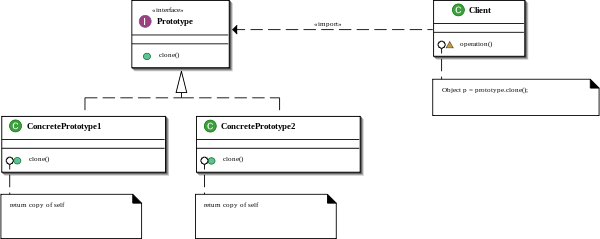
\includegraphics[width=0.9\textwidth]{content/gof/images/02-prototype-uml.png}
	\caption{Prototype UML}
\end{figure}


\section{Singleton}
\textbf{Kategorie}: Creational

Dieses Pattern stellt sicher, dass es von einer Klasse nur genau ein Objekt gibt und dieses global verfügbar ist.
Häufig wird es zum Beispiel für einen Logger oder ein Konfigurations-Objekt verwendet.

\begin{itemize}
	\item \textit{Nachteile:}
	\item exzessive Verwendung führt dazu, dass man quasi ein Äquivalent zu globalen Variablen erstellt und somit nicht mehr OOP macht
	\item Kopplung wird erhöht und die Abhängigkeiten zum Singleton sind nicht über das Interface klar
	\item Bei concurrent Applikationen wird es schwer, ein Singleton tatsächlich nur einmal zu erstellen
	\item Testen von Singletons kann sehr schwer sein (Mocken ist aufwändig)
\end{itemize}

\section{Factory Method}
\textbf{Kategorie}: Creational

Wenn Objekte erstellt werden müssen, ohne den exakten Typ (nur den einer Oberklasse) zu spezifizieren, kann eine Factory Method verwendet werden.
Je nach Subklasse erstellt die Factory Method ein anderes Objekt.

\begin{figure}[H]
	\centering
	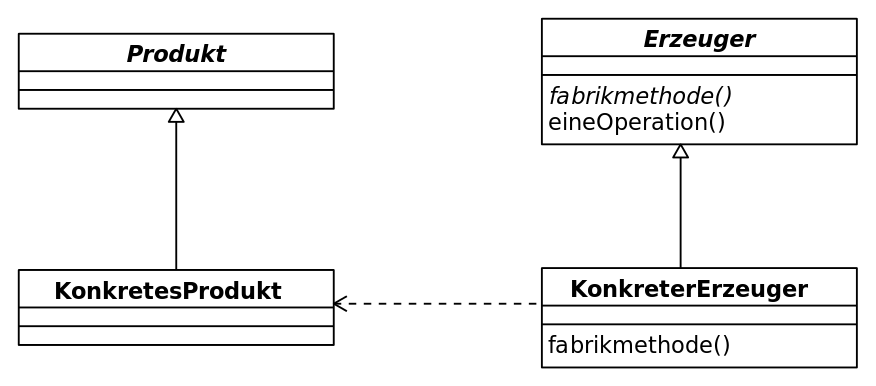
\includegraphics[width=0.9\textwidth]{content/gof/images/03-factory-method.png}
	\caption{Factory Method UML}
\end{figure}

\begin{lstlisting}[language=Java, caption={Factory Method}]
public class MazeGame {
	public MazeGame() {
		Room room1 = makeRoom();
		Room room2 = makeRoom();
		room1.connect(room2);
		this.addRoom(room1);
		this.addRoom(room2);
	}

	protected Room makeRoom() {
		return new OrdinaryRoom();
	}
}

// Do some magic ;)
public class MagicMazeGame extends MazeGame {
	@Override
	protected Room makeRoom() {
		return new MagicRoom();
	}
}
\end{lstlisting}

\section{Builder}

\textbf{Kategorie}: Creational

Wird verwendet um eine grosse Liste an Konstruktoren zu verhindern um ein Objekt zu erstellen. Der Builder bekommt step-by-step initialisierungs-Parameter und gibt schlussendlich das erstellte Objekt zurück.

\begin{figure}[H]
	\centering
	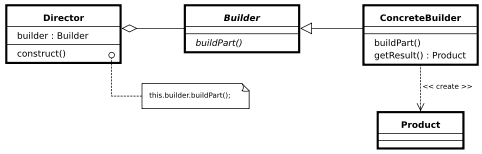
\includegraphics[width=0.9\textwidth]{content/gof/images/04-builder-uml.png}
	\caption{Builder UML}
\end{figure}


z.B. eine Auto-Klasse in der man verschiedene Einstellungen (Anzahl Sitze, Typ, mit/ohne GPS etc.) vornehmen kann. Dies wird mithilfe des Builders gesetzt. Nach vornehmen aller Einstellungen wird ein Auto-Objekt zurückgegeben, welcher alle gesetzten Einstellungen vorkonfiguriert hat.

\section{Adapter}
\textbf{Kategorie}: Structural

Dient zur Übersetzung eines Interfaces in ein anderes Interface. Dadurch wird die Kommunikation von Klassen mit inkompatiblen Schnittstellen vereinfacht/ermöglicht.


\subsection*{Implementation mit Delegation (Objektadapter)}

\begin{figure}[H]
	\centering
	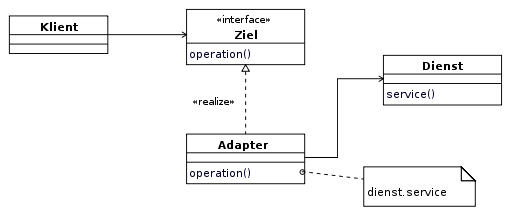
\includegraphics[width=0.9\textwidth]{content/gof/images/05-adapter-delegation-uml.png}
	\caption{Objektadapter UML}
\end{figure}


\begin{enumerate}
	\item Klasse wird an diese Instanz weitergeleitet.
\end{enumerate}


\subsection*{Implementation mit Vererbung (Klassenadapter)}

\begin{figure}[H]
	\centering
	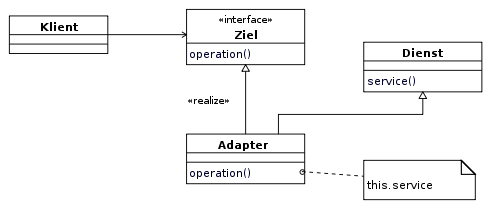
\includegraphics[width=0.9\textwidth]{content/gof/images/05-adapter-classes-uml.png}
	\caption{Klassendadapter UML}
\end{figure}

In dieser Variante wird mittels Mehrfachvererbung (sprich: in Java wäre es nur über ein weiteres Interface möglich) sowohl die Implementierung der zu adaptierenden Klasse wie auch die zu implementierende Schnittstelle geerbt.

\section{Bridge}
\textbf{Kategorie}: Structural

Dient zur Trennung der Implementierung von ihrer Abstraktion (Interface) wodurch beide unabhängig voneinander verändert werden können.

\begin{figure}[H]
	\centering
	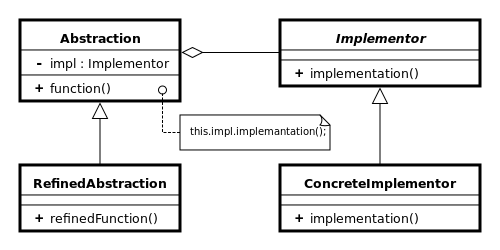
\includegraphics[width=0.9\textwidth]{content/gof/images/06-bridge-uml.png}
	\caption{Bridge UML}
\end{figure}

Im gezeigten UML hat die \textit{List} ein privates Feld namens \textit{impl}, welches beim Instanzieren zugewiesen wird. Jede public Methode wird in der \textit{List} an die entsprechende Implementierung weitergeleitet.

\section{Composite}
\textbf{Kategorie}: Structural

Das Composite Pattern wird angewendet um Teil-Ganzes-Hierarchien zu repräsentieren, indem Objekte zu Baumstrukturen zusammengefügt werden.

\begin{figure}[H]
	\centering
	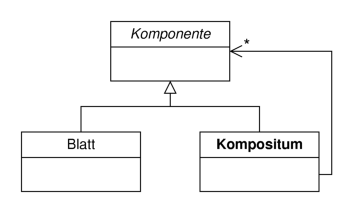
\includegraphics[width=0.9\textwidth]{content/gof/images/07-composite-uml.png}
	\caption{Composite UML}
\end{figure}


\section{Decorator}
\textbf{Kategorie}: Structural

Das Decorator Pattern erlaubt die Dekoration einer Komponente mit beliebig vielen anderen Klassen. Dies wird erreicht, in dem alle Klassen dasselbe Interface implementieren und eine entsprechende Methode überschreiben.

\begin{figure}[H]
	\centering
	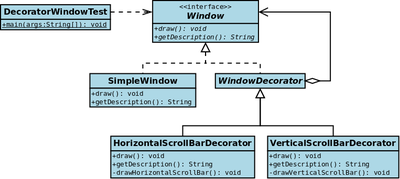
\includegraphics[width=0.9\textwidth]{content/gof/images/08-decorator-example-uml.png}
	\caption{Decorator UML}
\end{figure}


\section{Flyweight}
\textbf{Kategorie}: Structural

Wenn mehrere Objekte gleiche Datenstrukturen beinhalten ist es oftmals wünschenswert, diese in ein externes Objekt auszulagern, damit nicht unnötig RAM verwendet wird. Das Flyweight Pattern ist für diesen Zweck gedacht und wird z.B. bei einem Word processor verwendet, um nicht für jeden Character in einem Dokument die gleichen Informationen abspeichern zu müssen.

Um das Flyweight Objekt von mehreren Threads accessible machen zu können, muss es immutable sein.

\begin{figure}[H]
	\centering
	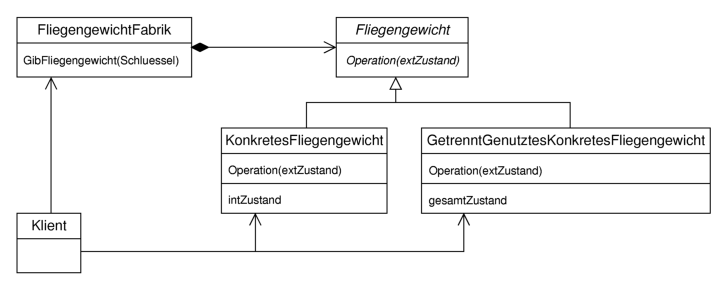
\includegraphics[width=0.9\textwidth]{content/gof/images/09-flyweight-uml.png}
	\caption{Flyweight UML}
\end{figure}

Innerhalb des Flyweight Patterns werden mehrere andere Patterns angewendet:

\begin{itemize}
	\item Immutable Value
	\item Factory Method als Teil eines Managers
	\item Pooling
\end{itemize}

\subsection*{Forces}

\begin{itemize}
	\item Es wird eine hohe Anzahl von Objekten benötigt
	\item Dadurch steigen die Speicherkosten
	\item Der Zustand der Objekte kann extrinsisch verwaltet werden (ausserhalb des Objekts selber, z.B. mit Collections for States)
	\item Viele Objekte können durch gemeinsam verwendete Objekte ersetzt werden, nachdem der Zustand entfernt wurde
	\item Die Identität der Objekte spielt keine Rolle (ValueObject)
\end{itemize}

\subsection*{Consequences}

\begin{itemize}
	\item Weniger Speicherverbrauch wird gegen einbussen der Runtime Performance ausgetauscht. Mehr Aufwand für das Auffinden der Objekte und der Verwaltung des extrinsischen Zustands.
	\item Je mehr Instanzen geteilt werden, desto weniger Speicher wird verbraucht.
	\item Zusätzliche Reduktion, wenn intrinsischer und extrinsischer Zustand auf ein Minimum reduziert werden können.
	\item Extrinsischer Zustand kann z.T. auch berechnet statt abgelegt werden.
	\item Flyweight kann oft zusammen mit dem Composite Pattern eingesetzt werden, wobei eine Hierarchie mit geteilten Blattknoten aufgebaut wird.
\end{itemize}

Extrinsischer Zustand kann zum Beispiel über das Collections for States Pattern oder über eine Map<Flyweight, ExtrinsicState> im Client verwaltet werden.

\section{Facade}
\textbf{Kategorie}: Structural

Eine Facade stellt ein Interface zu anderen APIs zur Verfügung. Es versucht die Benutzung einer API zu vereinfachen, oder auch zu verhindern, dass ein Client wissen muss, wo welcher Teil einer API implementiert wurde.

\begin{figure}[H]
	\centering
	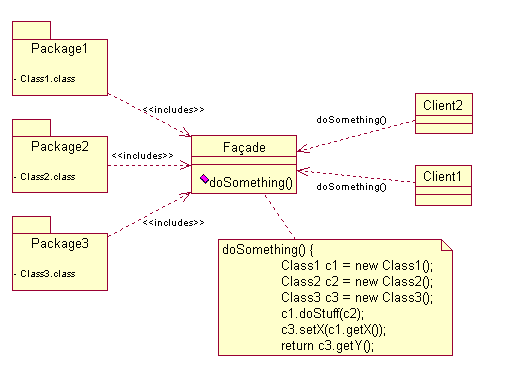
\includegraphics[width=0.9\textwidth]{content/gof/images/10-facade-uml.png}
	\caption{Facade UML}
\end{figure}


\section{Proxy}
\textbf{Kategorie}: Structural

Das Proxy Pattern wirkt als Stellvertreter für andere Objekte (Netzwerkverbindungen, ein grosses Objekt, eine Datei, etc.) und dient dazu, die Kontrolle vom eigentlichen Objekt zum Proxy-Objekt zu verschieben.

\begin{figure}[H]
	\centering
	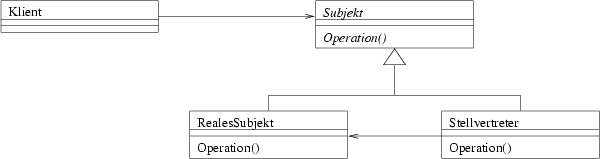
\includegraphics[width=0.9\textwidth]{content/gof/images/11-proxy-uml.png}
	\caption{Proxy UML}
\end{figure}


\section{Chain of Responsibility}
\textbf{Kategorie}: Behavioral

Das Chain of Responsibility Pattern beschreibt eine Kette von Objekten die miteinander verknüpft sind. Ein Beispiel ist z.B. ein Event-Handler, welcher einen Event abarbeiten muss. Jeder spezifische Event-Handler kann genau bestimmen, welche Events er verarbeiten möchte. Der Event-Handler wählt die Handlers aus welche sich auf diesen Event registriert haben und gibt der Reihe nach den Event weiter. Jeder Handler kann von sich aus bestimmen, ob er die Weiterreichung des Events zulassen möchte oder nicht.

\begin{figure}[H]
	\centering
	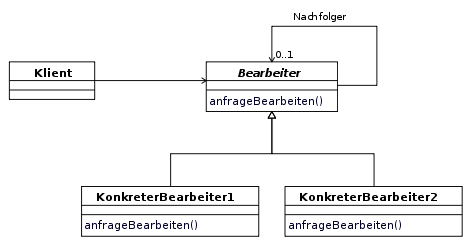
\includegraphics[width=0.9\textwidth]{content/gof/images/12-chain-of-responsibility-uml.png}
	\caption{Chain of Responsibility UML}
\end{figure}


\section{Command}
\textbf{Kategorie}: Behavioral

Das Command Pattern wird verwendet, um alle Informationen zu einem Methodenaufruf in einem Objekt zu speichern. Dies erlaubt den späteren nochmaligen Aufruf derselben Methode mit den gleichen Parametern etc.

\begin{figure}[H]
	\centering
	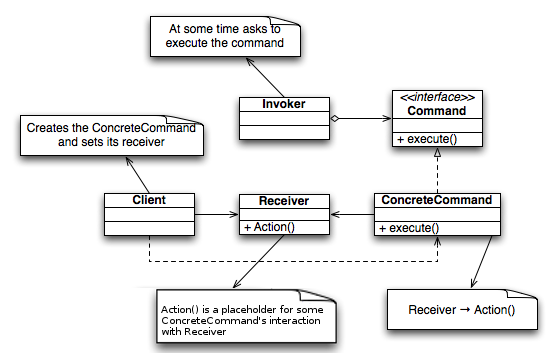
\includegraphics[width=0.9\textwidth]{content/gof/images/13-command-uml.png}
	\caption{Command UML}
\end{figure}


\section{Iterator}
\textbf{Kategorie}: Behavioral

Ein Iterator kann verwendet werden, um einen Container (bzw. dessen Elemente) zu traversieren. Er entkoppelt Algorithmus von Containern.

\section{Mediator}
\textbf{Kategorie}: Behavioral

Ein Mediator wird gebraucht um die Kommunikation zwischen Klassen zu entkoppeln und definiert somit ein Objekt, welches die Interaktion zwischen anderen Objekten kapselt.

\section{Memento}
\textbf{Kategorie}: Behavioral

Ermöglicht das Zurücksetzen von Objekten zum früheren Zustand (undo mit rollback).
Dies wird durch implementieren eines Memento Objekts erreicht, welches den Zustand bei jeder Zustandsänderung speichert. So kann zu jedem früheren Zustand wieder zurückgegangen werden.

\section{Observer}
\textbf{Kategorie}: Behavioral

Wird für distributed Event Handling Systeme verwendet. Ein Subjekt beinhaltet eine Collection an Observern. Wenn ein State Change passiert werden die Observer benachrichtigt (notify Methode).


\begin{figure}[H]
	\centering
	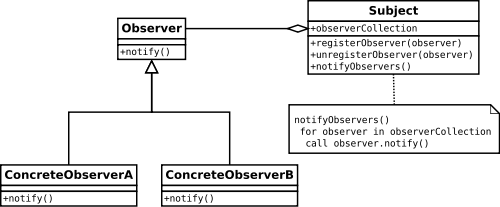
\includegraphics[width=0.9\textwidth]{content/gof/images/14-observer-uml.png}
	\caption{Observer UML}
\end{figure}


\section{State}
\textbf{Kategorie}: Behavioral

Ähnlich wie das Strategy Pattern implementiert ein Objekt mithilfe des State Patterns verschiedene Verhaltensweisen in der selben Routine aufgrund des Zustands eines Objekts. Damit können u.A. grosse Switch Statements verhindert werden.

\begin{figure}[H]
	\centering
	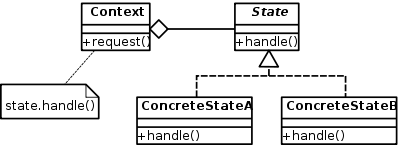
\includegraphics[width=0.9\textwidth]{content/gof/images/15-state-uml.png}
	\caption{State UML}
\end{figure}


\section{Strategy}
\textbf{Kategorie}: Behavioral

Das Strategy Pattern ermöglicht es zur Laufzeit die Implementation eines Algorithmus' auszutauschen.

\begin{figure}[H]
	\centering
	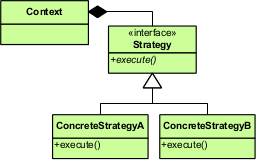
\includegraphics[width=0.9\textwidth]{content/gof/images/16-strategy-uml.png}
	\caption{Strategy UML}
\end{figure}


Der Context wird mit der gewünschten Strategy instanziert und darüber wird auch die Strategy dann ausgeführt.

\section{Visitor}
\textbf{Kategorie}: Behavioral

Wird verwendet um ein Algorithmus von der Objektstruktur auf welcher dieser arbeitet zu separieren.

\begin{figure}[H]
	\centering
	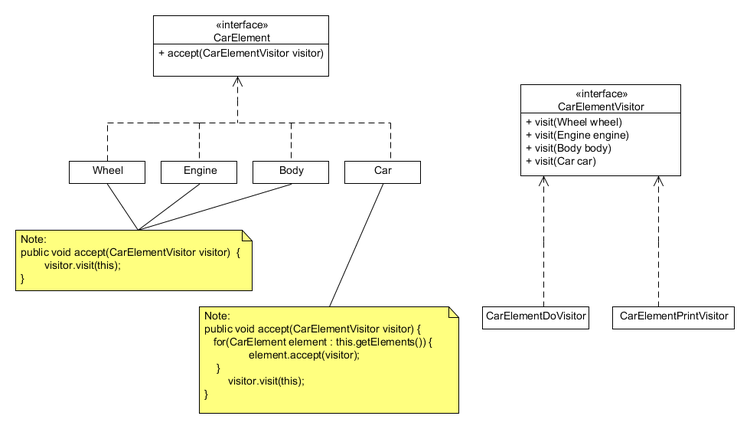
\includegraphics[width=0.9\textwidth]{content/gof/images/17-visitor-uml.png}
	\caption{Visitor UML}
\end{figure}


Die konkreten CarElementVisitor in diesem Fall implementiere die spezifische Funktionalität pro CarElement.
Der ``Client'' von aussen muss schlussendlich auf dem Car noch ein \textit{``car.accept(gewünschterVisitor)''} aufrufen, damit der Visitor startet.


\section{Template Method}
\textbf{Kategorie}: Behavioral

Eine Template Method implementiert mehrere Teile einer Methode selber und delegiert aber einzelne andere Teile in Subklassen. So können einzelne Teile spezifisch implementiert werden, ohne aber einen ganzen Algorithmus ändern zu müssen.

\begin{figure}[H]
	\centering
	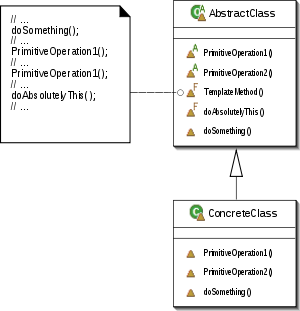
\includegraphics[width=0.9\textwidth]{content/gof/images/18-template-method-uml.png}
	\caption{Template Method UML}
\end{figure}


